\begin{frame}
	\frametitle{Example 1.}
	\framesubtitle{The Periodic Table}

	\begin{columns}
	\begin{column}{0.5\textwidth}
		\begin{itemize}
			\item<1-> In 1865, Mendeleev proposed that elements be ordered into the periodic table.
			\item<2-> He left gaps in the table, where his theory predicted there should be new matter.
			\item<3-> When these elements were discovered, he was hailed as a scientific hero.
		\end{itemize}
	\end{column}
	\begin{column}{0.5\textwidth}

	\begin{tikzpicture}
	  	\node (img1) {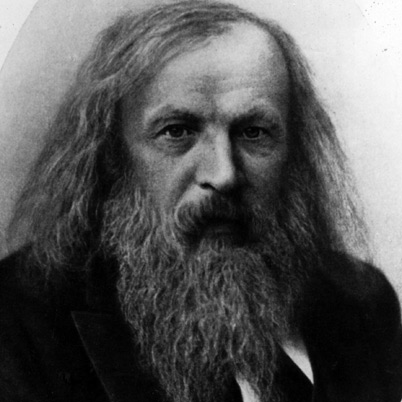
\includegraphics[height=4cm]{Images/mendeleev.jpg}};
	  	\pause
		\node (img2) at (img1.south) [yshift=-1cm] {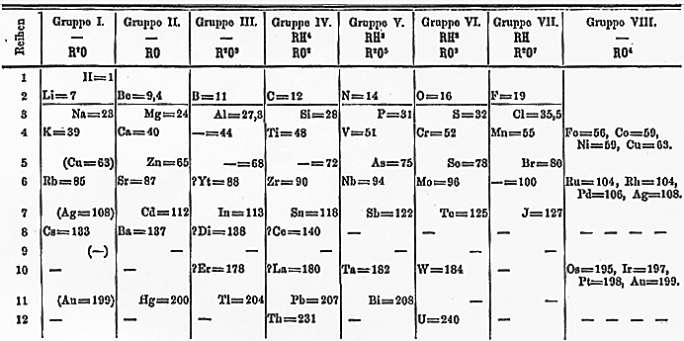
\includegraphics[width=\textwidth]{Images/periodic_table.png}};
	\end{tikzpicture}

	\end{column}
	\end{columns}
\end{frame}

\begin{frame}
	\frametitle{Example 2.}
	\framesubtitle{Orbits of Uranus and Mercury}

	\begin{columns}
	\begin{column}{0.5\textwidth}
		\includegraphics<1->[width=\textwidth]{Images/uranus.png}
		\begin{itemize}
			\item<1-> In 1841, it was noticed that Uranus' orbit was slightly off from predictions. 
			\item<2-> This observation led to the discovery of Neptune in 1846.
		\end{itemize}
	\end{column}
	\begin{column}{0.5\textwidth}
		\includegraphics<3->[width=\textwidth]{Images/mercury.jpg}
		\begin{itemize}
			\item<3-> In 1859, a similar problem emerged with the orbit of mercury
			\item<4-> This issue wasn't solved until Einstein's theory of general relativity superseded Newton's gravity in 1915.
		\end{itemize}


	\end{column}
	\end{columns}
\end{frame}



